% VAM Reformulering van het Standaardmodel-Lagrangian
% Alle termen zijn uitgedrukt in VAM-basiseenheden: Ce, rc, rho_ae, F_max

\documentclass{article}
\usepackage{amsmath,amssymb,graphicx}
\usepackage[margin=1in]{geometry}
\usepackage[backend=biber,style=phys]{biblatex}
\addbibresource{referenced.bib}

\title{Standaardmodel-Lagrangian in Vortex \AE ther Model-Eenheden}
\author{Omar Iskandarani}
\date{Mei 2025}
\begin{document}

    \maketitle

    \section*{Inleiding}
    Het standaardmodel van de deeltjesfysica kan worden geherformuleerd met behulp van de fundamentele constanten van het Vortex \AE ther Model (VAM):
    \begin{itemize}
        \item $C_e$: tangentiële snelheid in de wervelkern (wervelsnelheid)
        \item $r_c$: straal van de wervelkern (minimale circulatieschaal)
        \item $\rho_\ae$: dichtheid van de \ae ther (massa per volume)
        \item $F_{\text{max}}$: maximale interactiekracht binnen de \ae ther
    \end{itemize}
    Deze constanten definiëren een nieuw natuurlijk eenhedensysteem waarin energie, massa en tijd voortkomen uit vloeistofachtige beweging en topologische structuur.

    \section*{Geherformuleerde Lagrangian in VAM-Eenheden}
    \begin{align*}
        \mathcal{L}_{\text{VAM}} &= \underbrace{\sum_{a}\left( -\frac{1}{4} F^{a}_{\mu\nu} F^{a\mu\nu} \right)}_{\text{\textbf{Wervelveldenergie}: spanning en koppeling}} \\
        &+ \underbrace{\sum_{f} i(m_f C_e r_c) \bar{\psi}_f \gamma^\mu D_\mu \psi_f}_{\text{\textbf{Fermion-inertie}: massa uit werveltraagheid}} \\
        &- \underbrace{\left| D_\mu \phi \right|^2}_{\text{\textbf{\AE therweerstand}: elasticiteit tegen verstoring}} \\
        &- \underbrace{\left( - \frac{F_{\text{max}}}{r_c} |\phi|^2 + \lambda |\phi|^4 \right)}_{\text{\textbf{Drukpotentiaal}: wervel-evenwicht}} \\
        &- \underbrace{\sum_f \left( y_f \bar{\psi}_f \phi \psi_f + \text{h.c.} \right)}_{\text{\textbf{Toegevoegde massa}: interactie door drukweerstand}} \\
        &+ \underbrace{\text{topologische heliciteitstermen}}_{\text{\textbf{Wervelkoppeling}: knopen, verbinden, draaien}}
    \end{align*}

    \section*{Basisgrootheden in VAM-Eenheden}
    \begin{align*}
        L_0 &= r_c \quad \text{(lengte)} \\
        T_0 &= \frac{r_c}{C_e} \quad \text{(tijd)} \\
        M_0 &= \frac{F_{\text{max}} r_c}{C_e^2} \quad \text{(massa)} \\
        E_0 &= F_{\text{max}} r_c \quad \text{(energie)}
    \end{align*}

    \section*{Afgeleide Constanten en Koppelingen}
    \begin{align*}
        \hbar_{\text{VAM}} &= m_e C_e r_c \\
        c &= \sqrt{\frac{2 F_{\text{max}} r_c}{m_e}} \quad \text{(lichtsnelheid als emergente golfsnelheid)} \\
        \alpha &= \frac{2 C_e}{c} \quad \text{(fijnstructuur)} \\
        e^2 &= 8\pi m_e C_e^2 r_c \\
        \Gamma &= 2\pi r_c C_e = \frac{h}{m_e} \\
        v &= \sqrt{\frac{F_{\text{max}} r_c^3}{C_e^2}} \quad \text{(Higgs-veldwaarde uit \ae therspanning)}
    \end{align*}

    \section*{Onderbouwende Experimentele en Theoretische Observaties}
    Het VAM-kader sluit aan bij een brede verzameling experimentele en theoretische studies die wervelstrekking, heliciteitsbehoud en massa-energie-equivalentie bevestigen:

    \begin{itemize}
        \item Batchelor (1953): Strekking van wervellijnen in turbulente stroming verkleint de kernstraal en verhoogt de swirl~\cite{batchelor1953}.
        \item Vinen (2002): Kwantumwervels in supervloeibaar helium strekken onder axiale spanning~\cite{vinen2002}.
        \item Bewley et al. (2008): Visualisatie van reconnectie en dunner worden van kwantumwervels in helium II~\cite{bewley2008}.
        \item Moffatt (1969): Helicititeit als behoudende grootheid in geknoopte wervels~\cite{moffatt1969}.
        \item Irvine et al. (2013–2018): Geknoopte wervelstructuren in vloeistof behouden heliciteit en tonen rek- en verbindingsdynamiek~\cite{kleckner2013,scheeler2014}.
        \item Bartlett \& van Buren (1986): Massa als gevolg van inwendige structurele spanning, analoog aan wervelinertie~\cite{bartlett1986}.
    \end{itemize}

    \section*{Wervelversnelling via Mechanische Koppeling}
    \begin{figure}[h!]
        \centering
        \includegraphics[width=0.65\textwidth]{c4825aa0-8e0b-446f-87ef-6320137a44ff.png}
        \caption{Mechanisch model van een gekoppelde knoopwervel (gebaseerd op werk van Dr. Saul Schleimer en Henry Segerman). De draaiende knoop koppelt aan een axiale schroefdraadstructuur en induceert polaire stroming. Dit is een fysiek analogon van tijdsverloop en traagheid binnen het Vortex \AE ther Model.}
    \end{figure}

    \section*{Visualisatie van Wervelknoop met Kernradius $r_c$}
    \begin{figure}[h!]
        \centering
        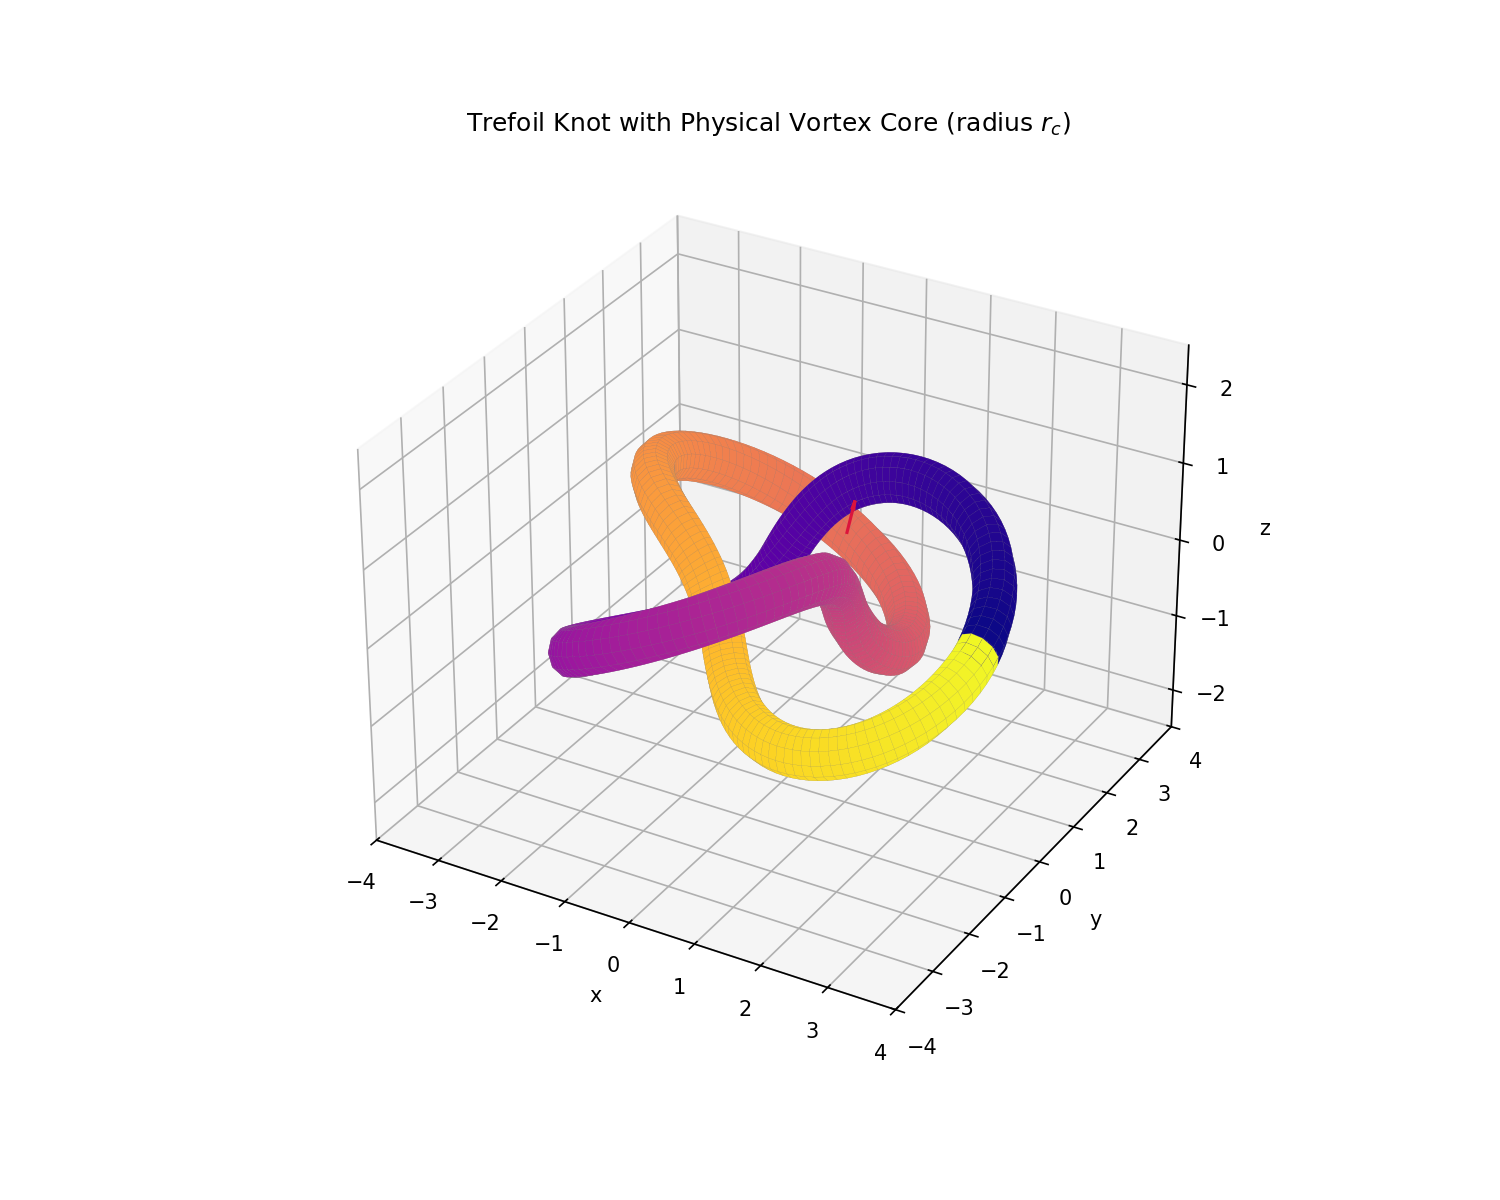
\includegraphics[width=0.8\textwidth]{FatTreFoil.png}
        \caption{Driedimensionale weergave van een dikke wervelknoop met fysieke kernstraal $r_c$, inclusief tangentiële snelheid $C_e$ (rood vectorveld).}
    \end{figure}

    \section*{Wervelknoop met Polaire Tijdsdraad}
    \begin{figure}[h!]
        \centering
        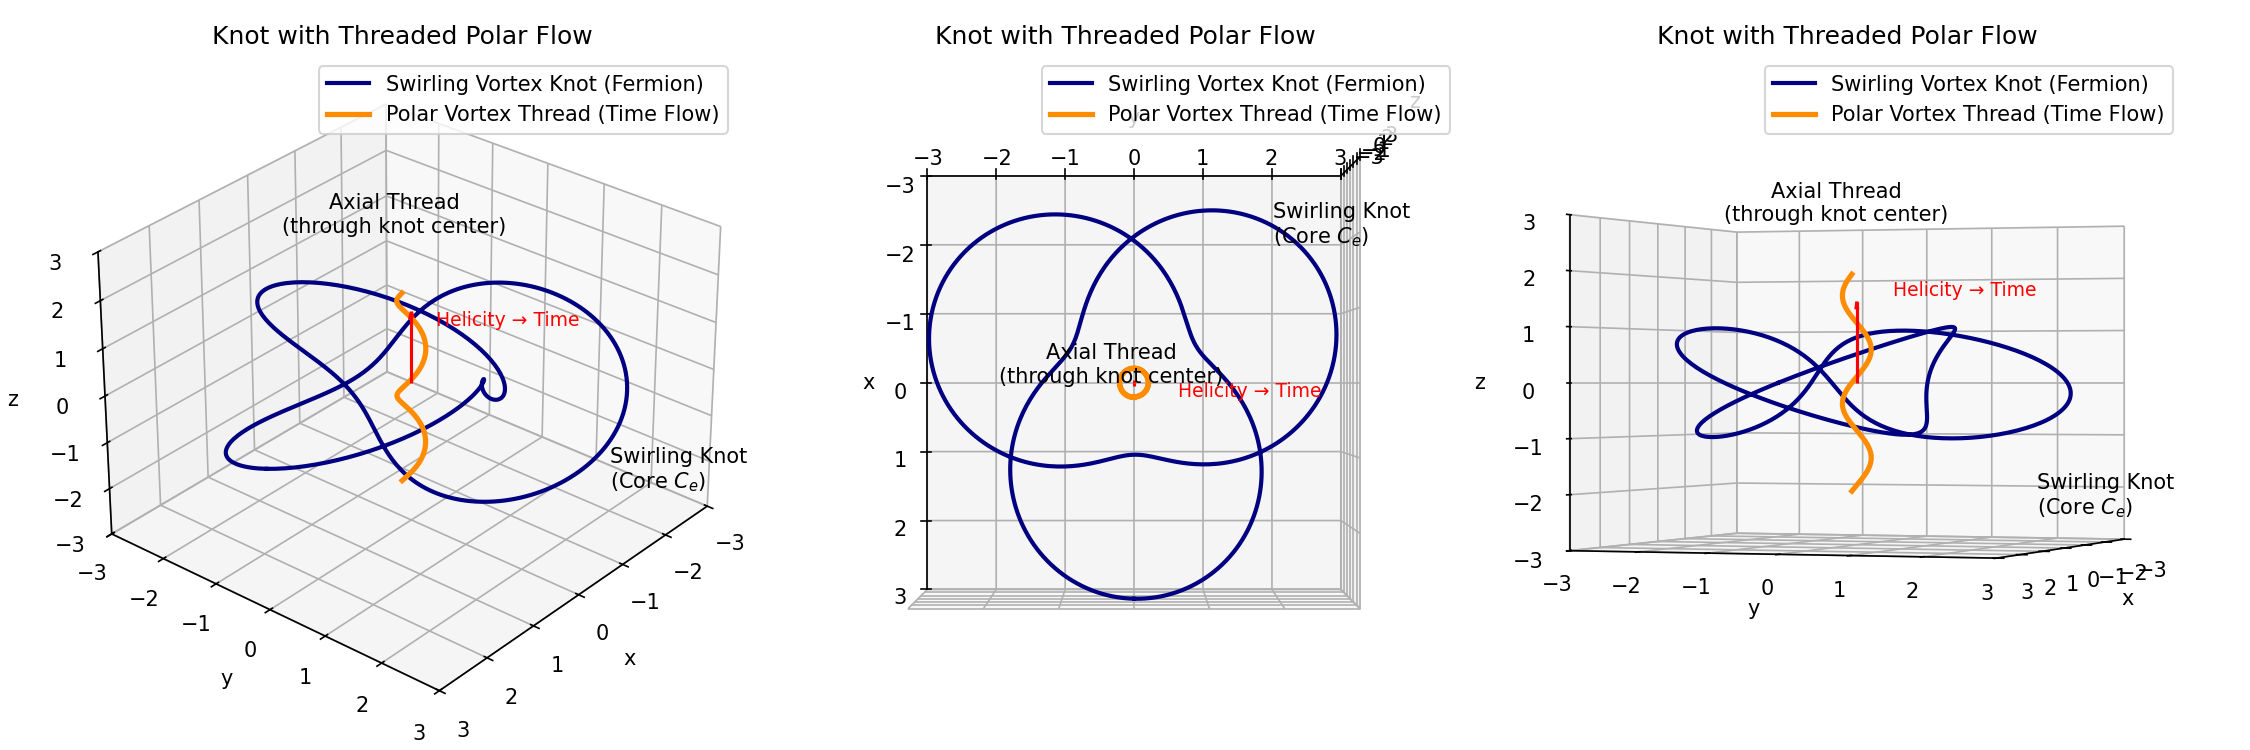
\includegraphics[width=0.98\textwidth]{KnotThreadedPolarFlow.png}
        \caption{Wervelknoop (blauw) gekoppeld aan een doorlopende polaire draad (oranje) — visualisatie van tijdsevolutie als heliciteitstransport. Links perspectivisch, midden-top, rechts-zijaanzicht.}
    \end{figure}

    \section*{Topologische Annotatie van Kernstraal}
    \begin{figure}[h!]
        \centering
        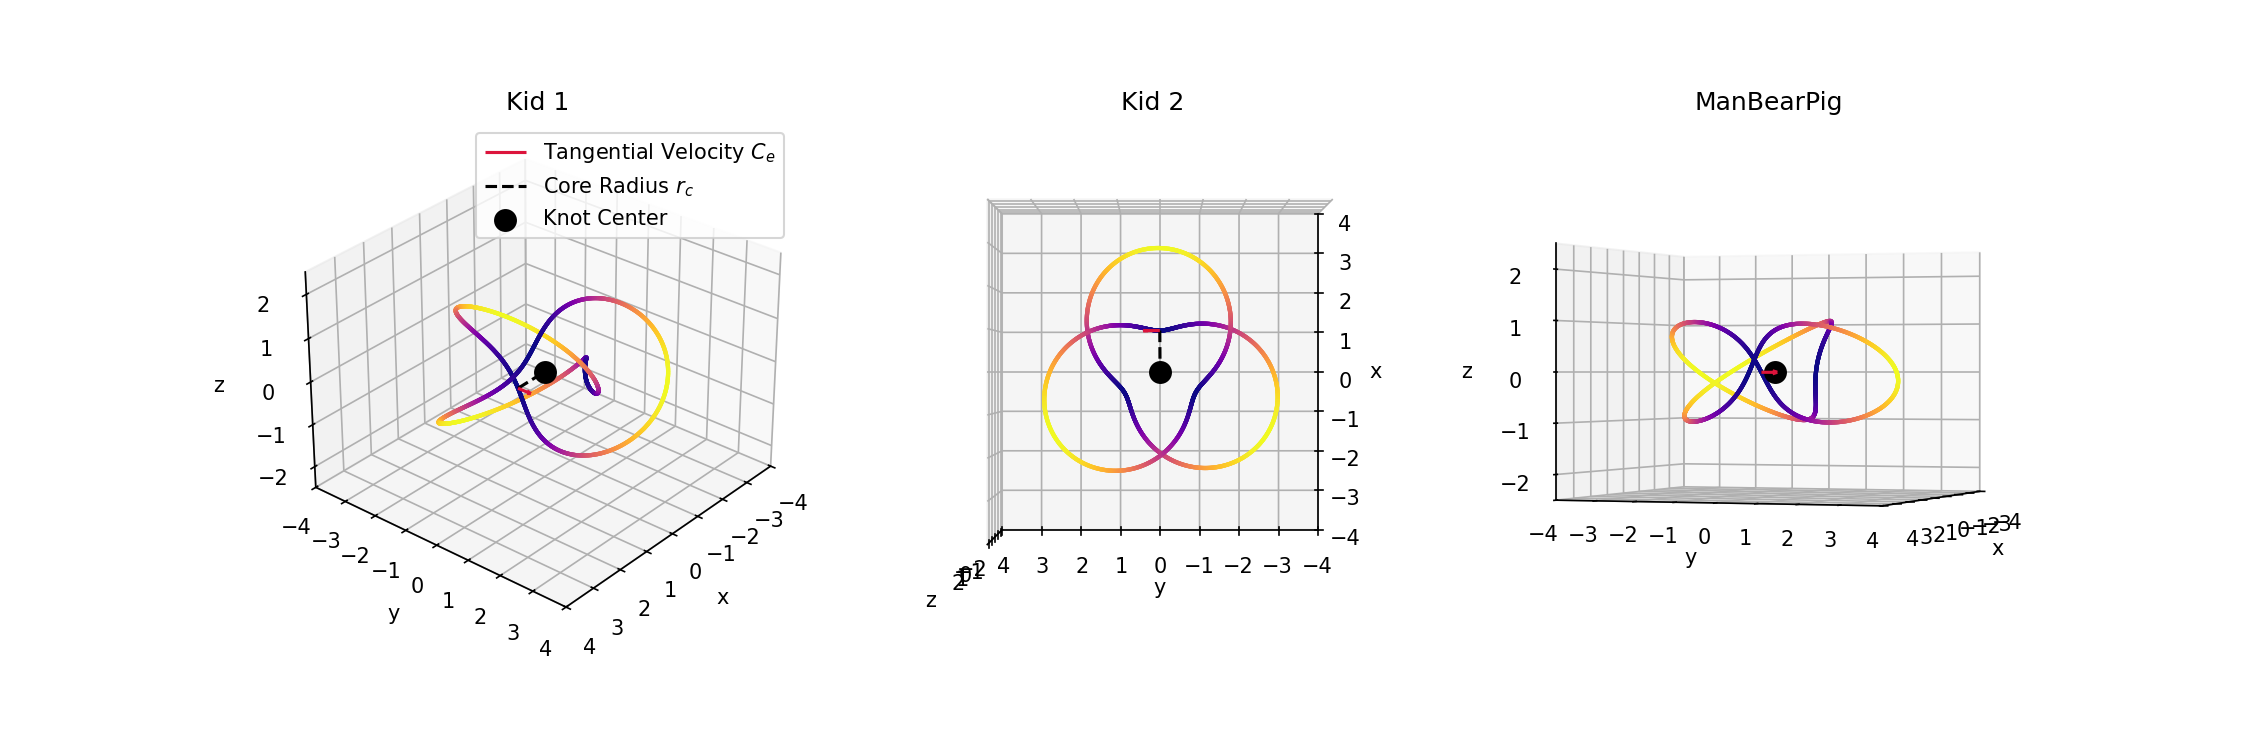
\includegraphics[width=0.95\textwidth]{vortex_knot_diagram.png}
        \caption{Annotatie van een gekleurde knoop met swirlgradient, kernstraal $r_c$ (stippellijn), centrum en swirlrichting $C_e$.}
    \end{figure}


    \section*{Overzichtstabel: Grootheden in VAM}

    \begin{table}[h!]
        \centering
        \begin{tabular}{|c|l|l|}
            \hline
            \textbf{Symbool} & \textbf{Beschrijving} & \textbf{Eenheid in VAM} \\
            \hline
            $C_e$ & Tangentiële wervelsnelheid (swirl) & $[L/T]$ \\
            $r_c$ & Straal van de wervelkern & $[L]$ \\
            $\rho_\ae$ & \AE therdichtheid & $[M/L^3]$ \\
            $F_{\text{max}}$ & Maximale kracht in de wervel & $[M \cdot L/T^2]$ \\
            $\Gamma$ & Circulatie (behouden) & $[L^2/T]$ \\
            $\hbar_{\text{VAM}}$ & Wervelmoment (vergelijkbaar met $\hbar$) & $[M \cdot L^2 / T]$ \\
            $E_0$ & Elementaire energie-eenheid & $[M \cdot L^2 / T^2]$ \\
            $T_0$ & Elementaire tijdseenheid & $[T]$ \\
            $L_0$ & Elementaire lengteeenheid & $[L]$ \\
            $M_0$ & Elementaire massa-eenheid & $[M]$ \\
            \hline
        \end{tabular}
        \caption{Overzicht van fundamentele grootheden in het Vortex \AE ther Model.}
    \end{table}

    \printbibliography

\end{document}